\documentclass[12pt, brazilian, a5paper]{abntex2} % Default font size and left-justified equations

%%%%%%%%%%%%%%%%%%%%%%%%%%%%%%%%%%%%%%%%%
% The Legrand Orange Book
% Structural Definitions File
% Version 2.1 (26/09/2018)
%
% Original author:
% Mathias Legrand (legrand.mathias@gmail.com) with modifications by:
% Vel (vel@latextemplates.com)
%
% This file was downloaded from:
% http://www.LaTeXTemplates.com
%
% License:
% CC BY-NC-SA 3.0 (http://creativecommons.org/licenses/by-nc-sa/3.0/)
%
%%%%%%%%%%%%%%%%%%%%%%%%%%%%%%%%%%%%%%%%%

% % ----------------------------------------------------------------------------------------
% %	VARIOUS REQUIRED PACKAGES AND CONFIGURATIONS
% % ----------------------------------------------------------------------------------------

% \hypersetup{pdftitle={Title},pdfauthor={Author}} % Uncomment and fill out to include PDF metadata for the author and title of the book

% \usepackage{mathtools}
% \usepackage{amsfonts}
% \usepackage{mathrsfs} % para mathscr

\usepackage{ifxetex}
\ifxetex
% % se for utilizar as fontes do sistema: **escolha sua fonte**
% comandos de fontes
\usepackage{mathspec}
\setmathsfont(Digits,Latin,Greek){Minion Pro}
\setmathrm{Minion Pro}
\setmainfont[Numbers=OldStyle]{Minion Pro} %fonte principal (serifada)
\setsansfont[Scale=0.9]{Myriad Pro} %fonte sem serifas
\setmonofont[Scale=MatchLowercase]{Consolas} % fonte monoespaçada

\usepackage{polyglossia} %always load polyblossia after fonts for digits in math mode
\setmainlanguage{brazil}
\setotherlanguages{french,english,spanish,german,italian}

\else
% % se for utilizar pdflatex
% \usepackage[utf8]{inputenc}
% \usepackage{newtxmath}
% \usepackage{Alegreya}
% \usepackage{AlegreyaSans}
\usepackage[nf]{coelacanth}
\usepackage[T1]{fontenc}
%% The font package uses mweights.sty which has som issues with the
%% \normalfont command. The following two lines fixes this issue.
\let\oldnormalfont\normalfont
\def\normalfont{\oldnormalfont\mdseries}
\usepackage[lf]{FiraMono}
\usepackage[italic]{mathastext}
\usepackage{slantsc}
\fi


%% Observação: o pacote polyglossia pode apresentar erro ao ser utilizado com ifxetex + babel.
%% Se isso acontecer, atualize o pacote para a versão mais recente ou utilize somente uma das sequências (pdflatex ou xelatex), comentando ou apagando a outra.

\usepackage{microtype} 				% para melhorias de justificação
% \usepackage[dvipsnames]{xcolor} 		% para cores
% \usepackage{graphicx} 			% para imagens
\usepackage{booktabs,tabularx,rotating}	% para tabelas
\usepackage{mdframed} 				% para caixas de texto como na CIP do verso do título
\usepackage{multicol}				% tabelas com colunas mescladas
\usepackage{lettrine}				% letras capitulares
\usepackage{xspace} 				% para nao precisar de espaços com {} depois de comandos
% como \LaTeX e abreviações criadas pelo usuário
\usepackage{lipsum} 				% para texto de preenchimento de exemplo
\usepackage{leading}				% espaçamento entrelinhas (leading)
\leading{13pt}

% ---
% Pacotes de citações
% ---
\usepackage[brazilian,hyperpageref]{backref}	 % Paginas com as citações na bibl
\usepackage[alf]{abntex2cite}	% Citações padrão ABNT

% ---
% Configurações do pacote backref
% Usado sem a opção hyperpageref de backref
\renewcommand{\backrefpagesname}{Citado na(s) página(s):~}
% Texto padrão antes do número das páginas
\renewcommand{\backref}{}
% Define os textos da citação
\renewcommand*{\backrefalt}[4]{
  \ifcase #1 %
  Nenhuma citação no texto.%
  \or
  Citado na página #2.%
  \else
  Citado #1 vezes nas páginas #2.%
  \fi}%
% ---


%% Spacing of general text; among lines, chapter, section etc
\setlength{\parindent}{1.3em}
\setlength{\parskip}{0.2em}
\renewcommand{\baselinestretch}{1.0}


\usepackage{graphicx} % Required for including pictures
\graphicspath{{Pictures/}} % Specifies the directory where pictures are stored

\usepackage{lipsum} % Inserts dummy text

\usepackage[edges]{forest}    %%Hierarchy Diagram
\usetikzlibrary{shadows.blur}

\usepackage{tikz} % Required for drawing custom shapes

% \usepackage[brazilian]{babel} % English language/hyphenation

\usepackage{enumitem} % Customize lists
\setlist{nolistsep} % Reduce spacing between bullet points and numbered lists

\usepackage{booktabs} % Required for nicer horizontal rules in tables

\usepackage{xcolor} % Required for specifying colors by name
\definecolor{ocre}{RGB}{243,102,25} % Define the orange color used for highlighting throughout the book

% % \usepackage{abntex2}

% % ----------------------------------------------------------------------------------------
% %	MARGINS
% % ----------------------------------------------------------------------------------------

\usepackage{geometry} % Required for adjusting page dimensions and margins

\geometry{
  paper=a4paper, % Paper size, change to letterpaper for US letter size
  top=2cm, % Top margin
  bottom=2cm, % Bottom margin
  left=2.3cm, % Left margin
  right=2.3cm, % Right margin
  headheight=3pt, % Header height
  footskip=1.5cm, % Space from the bottom margin to the baseline of the footer
  headsep=1cm, % Space from the top margin to the baseline of the header
  % showframe, % Uncomment to show how the type block is set on the page
}

% % ----------------------------------------------------------------------------------------
% %	FONTS
% % ----------------------------------------------------------------------------------------

% \usepackage{lmodern}	% Usa a fonte Latin Modern
% \usepackage{avant} % Use the Avantgarde font for headings
% % \usepackage{times} % Use the Times font for headings
% \usepackage{mathptmx} % Use the Adobe Times Roman as the default text font together with math symbols from the Sym­bol, Chancery and Com­puter Modern fonts

% \usepackage{microtype} % Slightly tweak font spacing for aesthetics
% \usepackage[utf8]{inputenc} % Required for including letters with accents
% \usepackage[T1]{fontenc} % Use 8-bit encoding that has 256 glyphs
\usepackage{indentfirst}		% Indenta o primeiro parágrafo de cada seção.

% % ----------------------------------------------------------------------------------------
% %	BIBLIOGRAPHY AND INDEX
% % ----------------------------------------------------------------------------------------

% \usepackage[style=numeric,citestyle=numeric,sorting=nyt,sortcites=true,autopunct=true,babel=hyphen,hyperref=true,abbreviate=false,backref=true,backend=biber]{biblatex}
% \addbibresource{bibliography} % BibTeX bibliography file
% \defbibheading{bibempty}{}

% ---
% Pacotes de citações
% ---
\usepackage[brazilian,hyperpageref]{backref}	 % Paginas com as citações na bibl
\usepackage[alf]{abntex2cite}	% Citações padrão ABNT
\usepackage{abntex2abrev}
% ---
% CONFIGURAÇÕES DE PACOTES
% ---

% ---
% Configurações do pacote backref
% Usado sem a opção hyperpageref de backref
\renewcommand{\backrefpagesname}{Citado na(s) página(s):~}
% Texto padrão antes do número das páginas
\renewcommand{\backref}{}
% Define os textos da citação
\renewcommand*{\backrefalt}[4]{
  \ifcase #1 %
  Nenhuma citação no texto.%
  \or
  Citado na página #2.%
  \else
  Citado #1 vezes nas páginas #2.%
  \fi}%
% ---

\usepackage{calc} % For simpler calculation - used for spacing the index letter headings correctly
\usepackage{makeidx} % Required to make an index
\makeindex % Tells LaTeX to create the files required for indexing

% ----------------------------------------------------------------------------------------
%	MAIN TABLE OF CONTENTS
% ----------------------------------------------------------------------------------------

\usepackage{titletoc} % Required for manipulating the table of contents

\contentsmargin{0cm} % Removes the default margin

% Part text styling (this is mostly taken care of in the PART HEADINGS section of this file)
\titlecontents{part}
[0cm] % Left indentation
{\addvspace{13pt}\bfseries} % Spacing and font options for parts
{}
{}
{}

% Chapter text styling
\titlecontents{chapter}
[1.25cm] % Left indentation
{\addvspace{20pt}\large\sffamily\bfseries} % Spacing and font options for chapters
{\color{ocre!60}\contentslabel[\Large\thecontentslabel]{1.5cm}\color{ocre}} % Formatting of numbered sections of this type
{\color{ocre}} % Formatting of numberless sections of this type
{\color{ocre!60}\normalsize\;\titlerule*[.5pc]{.}\;\thecontentspage}

% Formatting of the filler to the right of the heading and the
% page number

% Section text styling
\titlecontents{section}
[1.25cm] % Left indentation
{\addvspace{1pt}\sffamily\bfseries} % Spacing and font options for sections
{\contentslabel[\thecontentslabel]{1.25cm}} % Formatting of numbered sections of this type
{} % Formatting of numberless sections of this type
{\hfill\color{black}\thecontentspage} % Formatting of the filler to the right of the heading and the page number

% Subsection text styling
\titlecontents{subsection}
[1.25cm] % Left indentation
{\addvspace{1pt}\sffamily\small} % Spacing and font options for subsections
{\contentslabel[\thecontentslabel]{1.25cm}} % Formatting of numbered sections of this type
{} % Formatting of numberless sections of this type
{\ \titlerule*[.5pc]{.}\;\thecontentspage} % Formatting of the filler to the right of the heading and the page number

% Figure text styling
\titlecontents{figure}
[1.25cm] % Left indentation
{\addvspace{1pt}\sffamily\small} % Spacing and font options for figures
{\thecontentslabel\hspace*{1em}} % Formatting of numbered sections of this type
{} % Formatting of numberless sections of this type
{\ \titlerule*[.5pc]{.}\;\thecontentspage} % Formatting of the filler to the right of the heading and the page number

% Table text styling
\titlecontents{table}
[1.25cm] % Left indentation
{\addvspace{1pt}\sffamily\small} % Spacing and font options for tables
{\thecontentslabel\hspace*{1em}} % Formatting of numbered sections of this type
{} % Formatting of numberless sections of this type
{\ \titlerule*[.5pc]{.}\;\thecontentspage} % Formatting of the filler to the right of the heading and the page number

% ----------------------------------------------------------------------------------------
%	MINI TABLE OF CONTENTS IN PART HEADS
% ----------------------------------------------------------------------------------------

% Chapter text styling
\titlecontents{lchapter}
[0em] % Left indentation
{\addvspace{15pt}\large\sffamily\bfseries} % Spacing and font options for chapters
{\color{ocre}\contentslabel[\Large\thecontentslabel]{1.25cm}\color{ocre}} % Chapter number
{}
{\color{ocre}\normalsize\sffamily\bfseries\;\titlerule*[.5pc]{.}\;\thecontentspage} % Page number

% % Section text styling
\titlecontents{lsection}
[0em] % Left indentation
{\sffamily\small} % Spacing and font options for sections
{\contentslabel[\thecontentslabel]{1.25cm}} % Section number
{}
{}

% Subsection text styling (note these aren't shown by default, display them by searchings this file for tocdepth and reading the commented text)
\titlecontents{lsubsection}
[.5em] % Left indentation
{\sffamily\footnotesize} % Spacing and font options for subsections
{\contentslabel[\thecontentslabel]{1.25cm}}
{}
{}

% ----------------------------------------------------------------------------------------
%	HEADERS AND FOOTERS
% ----------------------------------------------------------------------------------------

\usepackage{fancyhdr} % Required for header and footer configuration

\pagestyle{fancy} % Enable the custom headers and footers

\renewcommand{\chaptermark}[1]{\markboth{\sffamily\large\bfseries\chaptername\
    \thechapter.\ #1}{}} % Styling for the current chapter in the header
\renewcommand{\sectionmark}[1]{\markright{\sffamily\large\thesection\hspace{2pt}#1}{}} % Styling for the current section in the header

\fancyhf{} % Clear default headers and footers
\fancyhead[LE,RO]{\sffamily\large\thepage} % Styling for the page number in the header
\fancyhead[LO]{\rightmark} % Print the nearest section name on the left side of odd pages
\fancyhead[RE]{\leftmark} % Print the current chapter name on the right side of even pages
\fancyfoot[C]{\thepage} % Uncomment to include a footer

\renewcommand{\headrulewidth}{0.8pt} % Thickness of the rule under the header

\fancypagestyle{plain}{% Style for when a plain pagestyle is specified
  \fancyhead{}\renewcommand{\headrulewidth}{0pt}%
}

% Removes the header from odd empty pages at the end of chapters
\makeatletter
\renewcommand{\cleardoublepage}{
  \clearpage\ifodd\c@page\else
  \hbox{}
  \vspace*{\fill}
  \thispagestyle{empty}
  \newpage
  \fi}

% ----------------------------------------------------------------------------------------
%	THEOREM STYLES
% ----------------------------------------------------------------------------------------

\usepackage{amsmath,amsfonts,amssymb,amsthm} % For math equations, theorems, symbols, etc

\newcommand{\intoo}[2]{\mathopen{]}#1\,;#2\mathclose{[}}
\newcommand{\ud}{\mathop{\mathrm{{}d}}\mathopen{}}
\newcommand{\intff}[2]{\mathopen{[}#1\,;#2\mathclose{]}}
\renewcommand{\qedsymbol}{$\blacksquare$}
\newtheorem{notation}{Notation}[chapter]

% Boxed/framed environments
\newtheoremstyle{ocrenumbox}% Theorem style name
{0pt}% Space above
{0pt}% Space below
{\normalfont}% Body font
{}% Indent amount
{\small\bf\sffamily\color{ocre}}% Theorem head font
{\;}% Punctuation after theorem head
{0.25em}% Space after theorem head
{\small\sffamily\color{ocre}\thmname{#1}\nobreakspace\thmnumber{\@ifnotempty{#1}{}\@upn{#2}}% Theorem text (e.g. Theorem 2.1)
  \thmnote{\nobreakspace\the\thm@notefont\sffamily\bfseries\color{black}---\nobreakspace#3.}} % Optional theorem note

\newtheoremstyle{blacknumex}% Theorem style name
{5pt}% Space above
{5pt}% Space below
{\normalfont}% Body font
{} % Indent amount
{\small\bf\sffamily}% Theorem head font
{\;}% Punctuation after theorem head
{0.25em}% Space after theorem head
{\small\sffamily{\tiny\ensuremath{\blacksquare}}\nobreakspace\thmname{#1}\nobreakspace\thmnumber{\@ifnotempty{#1}{}\@upn{#2}}% Theorem text (e.g. Theorem 2.1)
  \thmnote{\nobreakspace\the\thm@notefont\sffamily\bfseries---\nobreakspace#3.}}% Optional theorem note

\newtheoremstyle{blacknumbox} % Theorem style name
{0pt}% Space above
{0pt}% Space below
{\normalfont}% Body font
{}% Indent amount
{\small\bf\sffamily}% Theorem head font
{\;}% Punctuation after theorem head
{0.25em}% Space after theorem head
{\small\sffamily\thmname{#1}\nobreakspace\thmnumber{\@ifnotempty{#1}{}\@upn{#2}}% Theorem text (e.g. Theorem 2.1)
  \thmnote{\nobreakspace\the\thm@notefont\sffamily\bfseries---\nobreakspace#3.}}% Optional theorem note

% Non-boxed/non-framed environments
\newtheoremstyle{ocrenum}% Theorem style name
{5pt}% Space above
{5pt}% Space below
{\normalfont}% Body font
{}% Indent amount
{\small\bf\sffamily\color{ocre}}% Theorem head font
{\;}% Punctuation after theorem head
{0.25em}% Space after theorem head
{\small\sffamily\color{ocre}\thmname{#1}\nobreakspace\thmnumber{\@ifnotempty{#1}{}\@upn{#2}}% Theorem text (e.g. Theorem 2.1)
  \thmnote{\nobreakspace\the\thm@notefont\sffamily\bfseries\color{black}---\nobreakspace#3.}} % Optional theorem note
\makeatother

% Defines the theorem text style for each type of theorem to one of the three styles above
\newcounter{dummy}
\numberwithin{dummy}{section}
\theoremstyle{ocrenumbox}
\newtheorem{theoremeT}[dummy]{Theorem}
\newtheorem{problem}{Problem}[chapter]
\newtheorem{exerciseT}{Exercise}[chapter]
\theoremstyle{blacknumex}
\newtheorem{exampleT}{Example}[chapter]
\theoremstyle{blacknumbox}
\newtheorem{vocabulary}{Vocabulary}[chapter]
\newtheorem{definitionT}{Definition}[section]
\newtheorem{corollaryT}[dummy]{Corollary}
\theoremstyle{ocrenum}
\newtheorem{proposition}[dummy]{Proposition}

% ----------------------------------------------------------------------------------------
%	DEFINITION OF COLORED BOXES
% ----------------------------------------------------------------------------------------

\RequirePackage[framemethod=default]{mdframed} % Required for creating the theorem, definition, exercise and corollary boxes
% Theorem box
\newmdenv[skipabove=7pt,
skipbelow=7pt,
backgroundcolor=black!5,
linecolor=ocre,
innerleftmargin=5pt,
innerrightmargin=5pt,
innertopmargin=5pt,
leftmargin=0cm,
rightmargin=0cm,
innerbottommargin=5pt]{tBox}

% Exercise box
\newmdenv[skipabove=7pt,
skipbelow=7pt,
rightline=false,
leftline=true,
topline=false,
bottomline=false,
backgroundcolor=ocre!10,
linecolor=ocre,
innerleftmargin=5pt,
innerrightmargin=5pt,
innertopmargin=5pt,
innerbottommargin=5pt,
leftmargin=0cm,
rightmargin=0cm,
linewidth=4pt]{eBox}

% Definition box
\newmdenv[skipabove=7pt,
skipbelow=7pt,
rightline=false,
leftline=true,
topline=false,
bottomline=false,
linecolor=ocre,
innerleftmargin=5pt,
innerrightmargin=5pt,
innertopmargin=0pt,
leftmargin=0cm,
rightmargin=0cm,
linewidth=4pt,
innerbottommargin=0pt]{dBox}

% Corollary box
\newmdenv[skipabove=7pt,
skipbelow=7pt,
rightline=false,
leftline=true,
topline=false,
bottomline=false,
linecolor=gray,
backgroundcolor=black!5,
innerleftmargin=5pt,
innerrightmargin=5pt,
innertopmargin=5pt,
leftmargin=0cm,
rightmargin=0cm,
linewidth=4pt,
innerbottommargin=5pt]{cBox}

% Creates an environment for each type of theorem and assigns it a theorem text style from the "Theorem Styles" section above and a colored box from above
\newenvironment{theorem}{\begin{tBox}\begin{theoremeT}}{\end{theoremeT}\end{tBox}}
\newenvironment{exercise}{\begin{eBox}\begin{exerciseT}}{\hfill{\color{ocre}\tiny\ensuremath{\blacksquare}}\end{exerciseT}\end{eBox}}
\newenvironment{definition}{\begin{dBox}\begin{definitionT}}{\end{definitionT}\end{dBox}}
\newenvironment{example}{\begin{exampleT}}{\hfill{\tiny\ensuremath{\blacksquare}}\end{exampleT}}
\newenvironment{corollary}{\begin{cBox}\begin{corollaryT}}{\end{corollaryT}\end{cBox}}

% ----------------------------------------------------------------------------------------
%	REMARK ENVIRONMENT
% ----------------------------------------------------------------------------------------

\newenvironment{remark}{%\par\vspace{10pt}\small % Vertical white space above the remark and smaller font size
  \begin{list}{}{
      \leftmargin=20pt % Indentation on the left
      \rightmargin=25pt}\item\ignorespaces % Indentation on the right
    \makebox[-2.5pt]{\begin{tikzpicture}[overlay]
        \node[draw=ocre!60,line width=1pt,circle,fill=ocre!25,font=\sffamily\bfseries,inner sep=2pt,outer sep=0pt] at (-15pt,0pt){\textcolor{ocre}{R}};\end{tikzpicture}} % Orange R in a circle
    \advance\baselineskip -1pt}{\end{list}\vskip5pt} % Tighter line spacing and white space after remark

% ----------------------------------------------------------------------------------------
%	SECTION NUMBERING IN THE MARGIN
% ----------------------------------------------------------------------------------------

\makeatletter
\renewcommand{\@seccntformat}[1]{\llap{\textcolor{ocre}{\csname the#1\endcsname}\hspace{1em}}}
\renewcommand{\section}{\@startsection{section}{1}{\z@}
  {-4ex \@plus -1ex \@minus -.4ex}
  {1ex \@plus.2ex }
  {\Large\scfamily\bfseries}}
\renewcommand{\subsection}{\@startsection {subsection}{2}{\z@}
  {-3ex \@plus -0.1ex \@minus -.4ex}
  {0.5ex \@plus.2ex }
  {\large\scfamily\bfseries}}
\renewcommand{\subsubsection}{\@startsection {subsubsection}{3}{\z@}
  {-2ex \@plus -0.1ex \@minus -.2ex}
  {.2ex \@plus.2ex }
  {\normalfont\large\scfamily\bfseries}}
\renewcommand\paragraph{\@startsection{paragraph}{4}{\z@}
  {-2ex \@plus-.2ex \@minus .2ex}
  {.1ex}
  {\normalfont\large\sffamily\bfseries}}

% ----------------------------------------------------------------------------------------
%	PART HEADINGS
% ----------------------------------------------------------------------------------------

% Numbered part in the table of contents
\newcommand{\@mypartnumtocformat}[2]{%
  \setlength\fboxsep{0pt}%
  \noindent\colorbox{ocre!20}{\strut\parbox[c][.7cm]{\ecart}{\color{ocre!70}\Large\sffamily\bfseries\centering#1}}\hskip\esp\colorbox{ocre!40}{\strut\parbox[c][0.7cm]{\linewidth-\ecart-\esp}{\Large\sffamily\centering#2}}%
}

% Unnumbered part in the table of contents
\newcommand{\@myparttocformat}[1]{%
  \setlength\fboxsep{4pt}%
  \noindent\colorbox{ocre!40}{\strut\parbox[c][0.7cm]{\linewidth}{\Large\sffamily\centering#1}}%
}

\newlength\esp
\setlength\esp{2pt}
\newlength\ecart
\setlength\ecart{0.2cm-\esp}
\newcommand{\thepartimage}{}%
\newcommand{\partimage}[1]{\renewcommand{\thepartimage}{#1}}%
\def\@part[#1]#2{%
  \ifnum \c@secnumdepth >-2\relax%
  \refstepcounter{part}%
  \addcontentsline{toc}{part}{\texorpdfstring{\protect\@mypartnumtocformat{\thepart}{#1}}{\partname~\thepart\ ---\ #1}}
  \else%
  \addcontentsline{toc}{part}{\texorpdfstring{\protect\@myparttocformat{#1}}{#1}}%
  \fi%
  \startcontents%
  \markboth{}{}%
  {\thispagestyle{empty}%
    \begin{tikzpicture}[remember picture,overlay]%
      \node at (current page.north west){\begin{tikzpicture}[remember picture,overlay]%
          \fill[ocre!20](0cm,0cm) rectangle (\paperwidth,-\paperheight);
          \node[anchor=north] at (4cm,-3.25cm){\color{ocre!60}\fontsize{500}{700}\sffamily\bfseries\thepart};
          \node[anchor=south east] at (\paperwidth-2cm,-\paperheight+1cm){\parbox[][][t]{14cm}{
              \printcontents{a}{0}{\setcounter{tocdepth}{4}}% The depth to which the Part mini table of contents displays headings; 0 for chapters only, 1 for chapters and sections and 2 for chapters, sections and subsections
            }};
          \node[anchor=north east] at
          (\paperwidth-3cm,-3.25cm){\parbox[t][][t]{10cm}{\strut\raggedleft\color{white}\fontsize{40}{50}\ttfamily\bfseries#2}};
          %%Parte structure, font, size
        \end{tikzpicture}};
    \end{tikzpicture}}%
  \@endpart}
\def\@spart#1{%
  \startcontents%
  \phantomsection
  {\thispagestyle{empty}%
    \begin{tikzpicture}[remember picture,overlay]%
      \node at (current page.north west){\begin{tikzpicture}[remember picture,overlay]%
          \fill[ocre!40](5cm,5cm) rectangle (\paperwidth,-\paperheight);
          \node[anchor=north east] at (\paperwidth-1.5cm,-3.25cm){\parbox[t][][t]{15cm}{\strut\raggedleft\color{white}\fontsize{30}{30}\sffamily\bfseries#1}};
        \end{tikzpicture}};
    \end{tikzpicture}}
  \addcontentsline{toc}{part}{\texorpdfstring{%
      \setlength\fboxsep{3pt}%
      \noindent\protect\colorbox{ocre!90}{\strut\protect\parbox[l][2cm]{\linewidth}{\Large\sffamily\protect\centering #1\quad\mbox{}}}}{#1}}%
  \@endpart}
\def\@endpart{\vfil\newpage
  \if@twoside
  \if@openright
  \null
  \thispagestyle{empty}%
  \newpage
  \fi
  \fi
  \if@tempswa
  \twocolumn
  \fi}

% ----------------------------------------------------------------------------------------
%	CHAPTER HEADINGS
% ----------------------------------------------------------------------------------------

% A switch to conditionally include a picture, implemented by Christian Hupfer
\newif\ifusechapterimage
\usechapterimagetrue
\newcommand{\thechapterimage}{}%
\newcommand{\chapterimage}[1]{\ifusechapterimage\renewcommand{\thechapterimage}{#1}\fi}%
\newcommand{\autodot}{.}
\def\@makechapterhead#1{%
  {\parindent \z@ \raggedright \normalfont
    \ifnum \c@secnumdepth >\m@ne
    \if@mainmatter
    \begin{tikzpicture}[remember picture,overlay]
      \node at (current page.north west)
      {\begin{tikzpicture}[remember picture,overlay]
          \node[anchor=north west,inner sep=0pt] at (0,0) {\ifusechapterimage\includegraphics[width=\paperwidth]{\thechapterimage}\fi};
          \draw[anchor=west] (\Gm@lmargin,-9cm) node [line width=2.3pt,rounded corners=15pt,draw=ocre,fill=white,fill opacity=0.7,inner sep=15pt]{\strut\makebox[22cm]{}};
          \draw[anchor=west] (\Gm@lmargin+.3cm,-9cm) node {\Large\sffamily\bfseries\color{black}\thechapter\autodot~#1\strut};
        \end{tikzpicture}};
    \end{tikzpicture}
    \else
    \begin{tikzpicture}[remember picture,overlay]
      \node at (current page.north west)
      {\begin{tikzpicture}[remember picture,overlay]
          \node[anchor=north west,inner sep=0pt] at (0,0) {\ifusechapterimage\includegraphics[width=\paperwidth]{\thechapterimage}\fi};
          \draw[anchor=west] (\Gm@lmargin,-8cm) node [line width=2pt,rounded corners=15pt,draw=ocre,fill=white,fill opacity=0.5,inner sep=15pt]{\strut\makebox[22cm]{}};
          \draw[anchor=west] (\Gm@lmargin+.3cm,-8cm) node {\normalsize\sffamily\bfseries\color{black}#1\strut};
        \end{tikzpicture}};
    \end{tikzpicture}
    \fi\fi\par\vspace*{270\p@}}}

% -------------------------------------------

\def\@makeschapterhead#1{%
  \begin{tikzpicture}[remember picture,overlay]
    \node at (current page.north west)
    {\begin{tikzpicture}[remember picture,overlay]
        \node[anchor=north west,inner sep=0pt] at (0,0) {\ifusechapterimage\includegraphics[width=\paperwidth]{\thechapterimage}\fi};
        \draw[anchor=west] (\Gm@lmargin,-9cm) node [line width=2pt,rounded corners=15pt,draw=ocre,fill=white,fill opacity=0.5,inner sep=15pt]{\strut\makebox[22cm]{}};
        \draw[anchor=west] (\Gm@lmargin+.3cm,-9cm) node {\normalsize\sffamily\bfseries\color{black}#1\strut};
      \end{tikzpicture}};
  \end{tikzpicture}
  \par\vspace*{270\p@}}
\makeatother

% ----------------------------------------------------------------------------------------
%	LINKS
% ----------------------------------------------------------------------------------------

\usepackage{hyperref}
\hypersetup{hidelinks,backref=true,pagebackref=true,hyperindex=true,colorlinks=false,breaklinks=true,urlcolor=ocre,bookmarks=true,bookmarksopen=false}

\usepackage{bookmark}
\bookmarksetup{
  open,
  numbered,
  addtohook={%
    \ifnum\bookmarkget{level}=0 % chapter
    \bookmarksetup{bold}%
    \fi
    \ifnum\bookmarkget{level}=-1 % part
    \bookmarksetup{color=ocre,bold}%
    \fi
  }
}



%% Spaces between Chapter, Section, Subsection etc and subsequent text
\usepackage{titlesec}
\titlespacing*{\section}
{2pt}{2ex plus 1ex minus .2ex}{3ex plus .3ex}
\titlespacing*{\subsection}
{2pt}{2ex plus 1ex minus .2ex}{3ex plus .3ex}

%% Chapter, Section, Subsection etc sizes

%%% Local Variables:
%%% mode: latex
%%% TeX-master: "livro"
%%% End:
 % Insert the commands.tex file which contains the majority of the structure behind the template


%% Identação modular no ambiente 'myparident'
\newlength\mystoreparindent
\newenvironment{myparindent}[1]{%
  \setlength{\mystoreparindent}{\the\parindent}
  \setlength{\parindent}{#1}
}{%
  \setlength{\parindent}{\mystoreparindent}
}

% ----------------------------------------------------------------------------------------

\begin{document}

% ----------------------------------------------------------------------------------------
%	TITLE PAGE
% ----------------------------------------------------------------------------------------

\begingroup
\thispagestyle{empty} % Suppress headers and footers on the title page
\begin{tikzpicture}[remember picture,overlay]
  \node[inner sep=0pt] (background) at (current page.center) {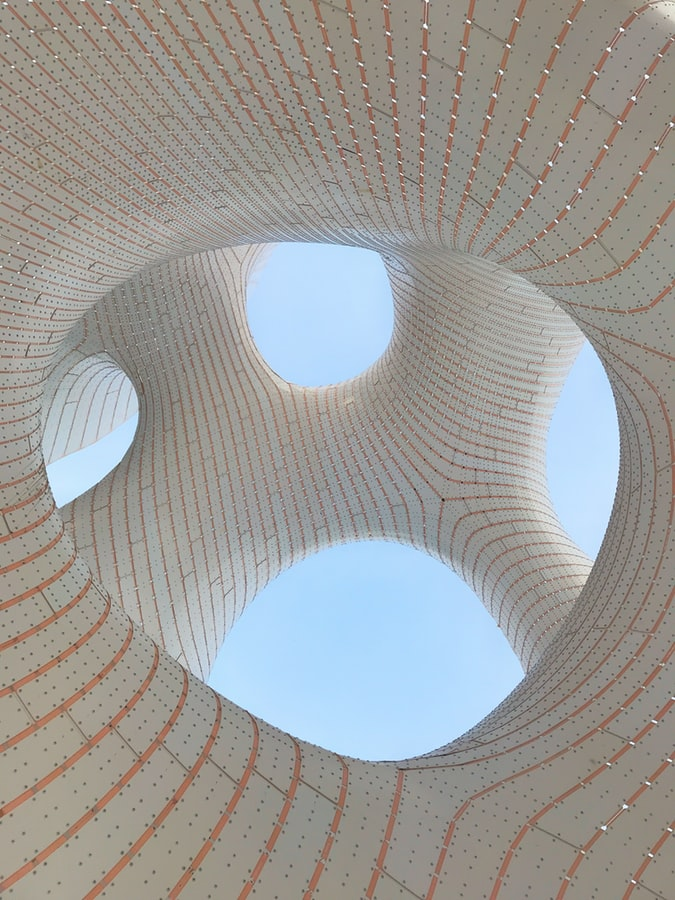
\includegraphics[width=\paperwidth]{005.jpeg}};
  \draw (current page.center) node [fill=ocre!30!white,fill
  opacity=0.6,text opacity=1,inner
  sep=1cm]{\Huge\centering\bfseries\sffamily\parbox[c][][t]{\paperwidth}{\centering
      Processador de Documentos: \LaTeX \\[15pt] % Book title
      {\Large Material Minicurso}\\[20pt] % Subtitle
      {\huge Aluno, Pedro G. Branquinho \\ Orientadora, Kátia C. G. Candioto}}}; % Author name
\end{tikzpicture}
\vfill
\endgroup

% ----------------------------------------------------------------------------------------
%	COPYRIGHT PAGE
% ----------------------------------------------------------------------------------------

\newpage
~\vfill
\thispagestyle{empty}

\noindent Copyright \copyright\ 2020 Pedro G. Branquinho\\ % Copyright notice

% \noindent \textsc{Published by BuddhiLWinc.}\\ % Publisher

\noindent \textsc{https://github.com/26-55-87-BuddhiLW/MC-LaTeX}\\ % URL

\noindent Licensed under the Creative Commons Attribution-NonCommercial 3.0 Unported License (the ``License''). You may not use this file except in compliance with the License. You may obtain a copy of the License at \url{http://creativecommons.org/licenses/by-nc/3.0}. Unless required by applicable law or agreed to in writing, software distributed under the License is distributed on an \textsc{``as is'' basis, without warranties or conditions of any kind}, either express or implied. See the License for the specific language governing permissions and limitations under the License.\\ % License information, replace this with your own license (if any)

% \noindent \textit{First printing, January 2020} % Printing/edition date
\clearpage
% ----------------------------------------------------------------------------------------
%	TABLE OF CONTENTS
% ----------------------------------------------------------------------------------------

% \usechapterimagefalse % If you don't want to include a chapter image, use this to toggle images off - it can be enabled later with \usechapterimagetrue

\chapterimage{16.jpg} % Table of contents heading image

\pagestyle{empty} % Disable headers and footers for the following pages

\tableofcontents % Print the table of contents itself

\cleardoublepage % Forces the first chapter to start on an odd page so it's on the right side of the book

\pagestyle{fancy} % Enable headers and footers again

% ----------------------------------------------------------------------------------------
%	PART
% ----------------------------------------------------------------------------------------

\part{Parte Um}

% ----------------------------------------------------------------------------------------
%	CHAPTER 1
% ----------------------------------------------------------------------------------------

\chapterimage{13.jpg} % Chapter heading image

\chapter{História e Filosofia do \LaTeX}
% \chapter{History and Philosophy of LaTeX}

% \section{LaTeX's Philosophy}\index{Philosophy}
\section{Paradigma do \LaTeX}\index{Filosofia}

% \subsection{Extensibility and Bottom-up Programming} \index{Extensibility and Bottom-up Programming}
\subsection{Extensibilidade e Programação Base-topo} \index{Extensibilidade e Programação Base-topo}
% ``Almost any program can benefit from having the language tailored to
% suit its needs, but the more complex the program, the more valuable
% bottom-up programming becomes. A bottom-up program can be written as a
% series of layers, each one acting as a sort of programming language
% for the one above. TeX was one of the earliest programs to be written
% this way.

% (...)Bottom-up programming leads to naturally extensible software. If
% you take the principle of bottom-up programming all the way up to the
% topmost layer of your program, then that layer becomes a programming
% language for the user.'' \cite{Graham1996}
``Quase qualquer programa pode se beneficiar ao ser escrito em uma linguagem feita à suas necessidades, ademais quanto mais complexo a programação, tanto mais valiosa é o paradigma base-topo de programação. Um programa escrito com esse paradigma pode ser feito de maneira progressiva, em camadas. Cada camada funcionando como um dialeto de comandos para camadas acima. A linguagem \TeX{} foi uma das primeiras a ser criada sob esse paradigma.

(...)Programação base-topo conduz a softwares naturalmente extensíveis. Se mantem-se a programação íntegra aos princípios de progração base-topo até suas últimas camadas, a última camada se torna uma linguagem de programação para o usuário.'' \cite{graham1995}



% For us to understand this, profoundly, we must understand some concepts.

% \begin{enumerate}
% \item What is bottom-up programming? What could it mean to have a language tailored
%   to suit our needs?

% \item  We must understand what a extensible software is.

% \item Finally, how the bottom-up programming leads to
%   extensible programs.
% \end{enumerate}

Para que entendamos essa citação, profundamente, devemos entender alguns conceitos chave.

\begin{enumerate}
\item O que é programação base-topo? O que significa ter uma linguagem creada para nossas necessidades?

\item Precisamos entender o que é um software estensível.

\item Finalmente, como o paradigma base-topo implica softwares estensíveis.
\end{enumerate}


% ``(...)Working bottom-up is also the best way to get reusable software.
% The essence of writing reusable software is to separate the general
% from the specific, and bottom-up programming inherently creates
% such a separation.  Instead of devoting all your effort to writing
% a single, monolithic application, you devote part of your effort
% to building a language, and part to writing a (proportionately
% smaller) application on top of it'' \cite{Graham1996}


``(...)Trabalhando-se de base à topo é também a melhor maneira de se adquirir softwares reutilizáveis. A essência de escrever um software reutilizável é separar o que é geral do que é específico, e a programação base-topo inerentemente cria tal divisão. Invés de se dedicar completamente a escrever uma, monolítica, aplicação, parte da programação vai para construir o dialeto e parte - proporcionalmente menor - é direcionada à escrita da aplicação baseada no dileto.'' \cite{graham1995}

% \subsection{Extensibility} \index{Extensibility}
% We will see later, in practice what is to build a 'language', and then
% build an 'application' on top of it. Suffice to say that, to us, to
% build a language is to design the format, the commands we will
% use. Therefore, 'language', in Graham's quote may be understood as the
% templates. The 'application' is your set of personal parameters set to
% the template, and
% the writing content of your work. This comprises our 'application',
% that is, your personal document.
\clearpage
\subsection{Extensibilidade} \index{Estensibilidade}
Veremos mais, posteriormente, o que significa, na prática, construir um dialeto, e então escrever sua aplicação, baseada nele. É suficiente, para nossos propósitos, traduzir a 'criação de um dialeto' por formatar, ou criar comandos dos quais utilizaremos para formatar um documento. Assim, 'dialeto', na citação de Graham pode ser interpretado como os \textit{templates} ou modelos. E, 'aplicação' nosso conjunto de parâmetros pessoais os quais delegamos aos templates, bem como o conteúdo textual dentro dos modelos. Isso compraz uma 'aplicação' do 'dialeto', isto é, o produto final é nosso documento.


%%

% Upon doing so, by applying, we just 'extended' the template to our use. And, your work, with
% other particular, local, programming, may be extended further, as a
% template. This in fact, will be the case of most of your works. Hardly
% ever will the user-developer start a document from scratch. Even in
% that case, he would use fundamental packages, and programming
% structures which would be an extension of the developers of these tools.

%%

Ao se fazer uma aplicação, nós estamos estendendo nosso \textit{template} ao nosso uso. E, nosso documento, com seus comandos forjados, particularmente, podem vir a ser estendidos adiante, como um prosseguinte 'modelo'. Essa estensão de modelos, de fato, será nossa dinâmica padrão para fazer uma aplicação. Raramente, iremos desenvolver um documento do início ao seu fim. Mesmo se planejamos fazer um documento extremamente personalizado, irríamos utilizar pacotes fundamentais, e por conseguinte, estruturas de programação das quais configuram como uma estensão de ferramentas feitas por outros autores-desenvolvedores.


% \subsection{Bottom-up Programming} \index{Bottom-up Programming}
% An didactic example of the endless extension behind a \LaTeX document
% is this book. I have built it, upon Mathias
% Legrand's template \footnote{Book Template: \url{
% https://www.latextemplates.com/template/the-legrand-orange-book}}. Legrands's
% template, in its turn, was extensively built from two sources
% \footnote{Source to the Legrand's template:
% \url{https://cel.archives-ouvertes.fr/cel-00814877/}} \footnote{Source to
% the Legrand's template: \url{http://pgoutet.free.fr/latex/}}, as
% documented by himself.

\subsection{Programando com Paradigma Base-topo} \index{Programação Base-topo}
Um exemplo didático da estensão indefinida, e recursiva, por trás das produções de documentos com \LaTeX, é a própria apostila. A apostila foi construida à partir do modelo de Mathias Legrand \footnote{Book Template: \url{
    https://www.latextemplates.com/template/the-legrand-orange-book}}. O modelo de Legrand, por sua vez, foi majoritariamente uma mistura de dois modelos
\footnote{Fontes estendidas por Legrand:
  \url{https://cel.archives-ouvertes.fr/cel-00814877/}} \footnote{Site onde se encontra o template de Legrand: \url{http://pgoutet.free.fr/latex/}}, como foi documentado pelo próprio autor.


%%


% At the same time, I mixed his template structure with the
% ABNT's norms, trough ABNTEX's package and templates
% \footnote{\url{https://github.com/abntex/abntex2}}. We may track down these sources to more fundamental sources. ABNTEX
% used extensively the Memoir Class
% \footnote{\url{http://linorg.usp.br/CTAN/macros/latex/contrib/memoir/memman.pdf}}.

% Therefore, this book may be visualized as a \textbf{bottom-up
% construction}. It has in it the history of older, more developed trough time, more deep,
% content. This work is only the top of the iceberg of all which goes
% behind it. Therefore, it's an bottom-up 'application' of this built 'language' structure.

Ao mesmo tempo, foi misturado a estrutura de seu template com as
normas ABNT, por meio dos pacotes ABNTeX e seus modelos
\footnote{\url{https://github.com/abntex/abntex2}}. Poderíamos, no
entanto, traçar fontes predecessoras às fontes supracitadas. Por
exemplo, o pacote ABNTeX foi construido em cima da Classe Memoir
\footnote{\url{http://linorg.usp.br/CTAN/macros/latex/contrib/memoir/memman.pdf}}.

Por conseguinte, esse livro pode ser visualizado como uma
\textbf{construção base-topo}. Está contido nele o desenvolvimento de
conteúdos indefinidamente mais abrangentes e trabalhados do que o
autor jamais poderia realizar sozinho. Isto é, por fim, o significado
de uma 'aplicação' base-topo desse específico 'dialeto', desenvolvido
como especializações de aplicações sucessivas da linguagem \TeX.


% \subsection{Tree Structure of This Book} \index{Tree Structure of This Book}
% \begin{center}
%   \begin{forest}
%     forked edges,
%     for tree={draw,align=center,edge={-latex}}
%     [Book Template's \\Structure
%     [Legrand and Vel's Book \\ Template
%     [Legrand's Article]
%     [Philippe Goutet's Minicourse
%     [Reference Books]
%     [Templates]
%     [Other Courses]
%     [Support Material]
%     ]
%     ]
%     [ABNTEX
%     [Memoir Class
%     [30 Packages]
%     ]
%     [ABNT norms]
%     ]
%     ]
%   \end{forest}
% \end{center}
\clearpage
\subsection{Estrutura em Árvore do Livro} \index{Estrutura em Árvore
  do livro}
\begin{center}
  \begin{forest}
    forked edges,
    for tree={draw,align=center,edge={-latex}}
    [Estrutura do Template \\do Livro
    [Template do Legrand e Vel \\ de seu Livro
    [Artigo do Legrand]
    [Minicurso de Philippe Goutet
    [Livros Referência]
    [Templates]
    [Outros cursos]
    [Materiais de Suporte]
    ]
    ]
    [ABNTEX
    [Memoir Class
    [30 Pacotes]
    ]
    [Normas ABNT]
    ]
    ]
  \end{forest}
\end{center}

% This is an image of how language extensibility imply bottom-up
% applications.

Essa é uma visualização de como a extensibilidade da língua implica
uma lógica de aplicação base-topo.



% ------------------------------------------------


% \section{LaTeX's History}\index{History}
\section{História do LaTeX}\index{História}

% \subsection{Leslie Lamport and Donald Knuth}
\subsection{Leslie Lamport e Donald Knuth}

% \LaTeX is an extensive build on \TeX language. It has used it's
% powerful macros to make producing high quality texts friendly. It's
% the work of Leslie Lamport, upon Donald Knuth's, which designed
% \TeX in the 80's. And, today, it counts with 34 years of extensive
% work and update of all the user-developer community.

% Lamport and Knuth are both Computer Scientists and
% Ph.D. Mathematicians. Their work extend far beyond \LaTeX and
% \TeX. They have contributed profoundly for the State of the Art of
% both fields. Both are receivers of many awards, including the Turing
% Award - one of the highest recognition awards on Computer Science.

\LaTeX{} é uma extensa construção em cima da linguagem \TeX. Foi o
resultado da utilização de poderosos macros. Com eles, foi possível
fazer com que a tipografia de textos de alto nível se tornassem
relativamente fáceis. Esse trabalho foi levado, inicialmente, por
Leslie Lamport, em cima do de Donald Knuth, o qual criou \TeX{} na
década de oitenta. E, hoje, conta com 34 anos de inquantificável
trabalho e atualização constante pela comunidade
usuário-desenvolvedora livre.

% Lamport and Knuth are both Computer Scientists and
% Ph.D. Mathematicians. Their work extend far beyond \LaTeX and
% \TeX. They have contributed profoundly for the State of the Art of
% both fields. Both are receivers of many awards, including the Turing
% Award - one of the highest recognition awards on Computer Science.

Lamport e Knuth são ambos Cientistas da Computação e
Ph.D. em Matemática. Seus trabalhos vão muito além do \LaTeX{} e
\TeX. Contribuiram, principalmente, para assuntos no estado da arte
em ambas áreas. Ambos receberam o prémio renomeado, Turing, em
computação.

\clearpage
\section{Sites de Referência}
\subsection{The Comprehensive TEX Archive Network (CTAN)}

CTAN é um repositório, com uma diversidade enorme de pacotes e
materiais sobre \TeX. E conta com mais de 5800 pacotes e 2600
contribuidores \footnote{https://www.ctan.org/}. O site aloja outros
sites primários, ou não, sobre LaTeX. O pacote ABNTeX2 se encontra nele, por exemplo.

\begin{figure}[!htb]
  \caption{\label{abntex_site} Procura do ABNTeX no CTAN}
  \begin{center}
    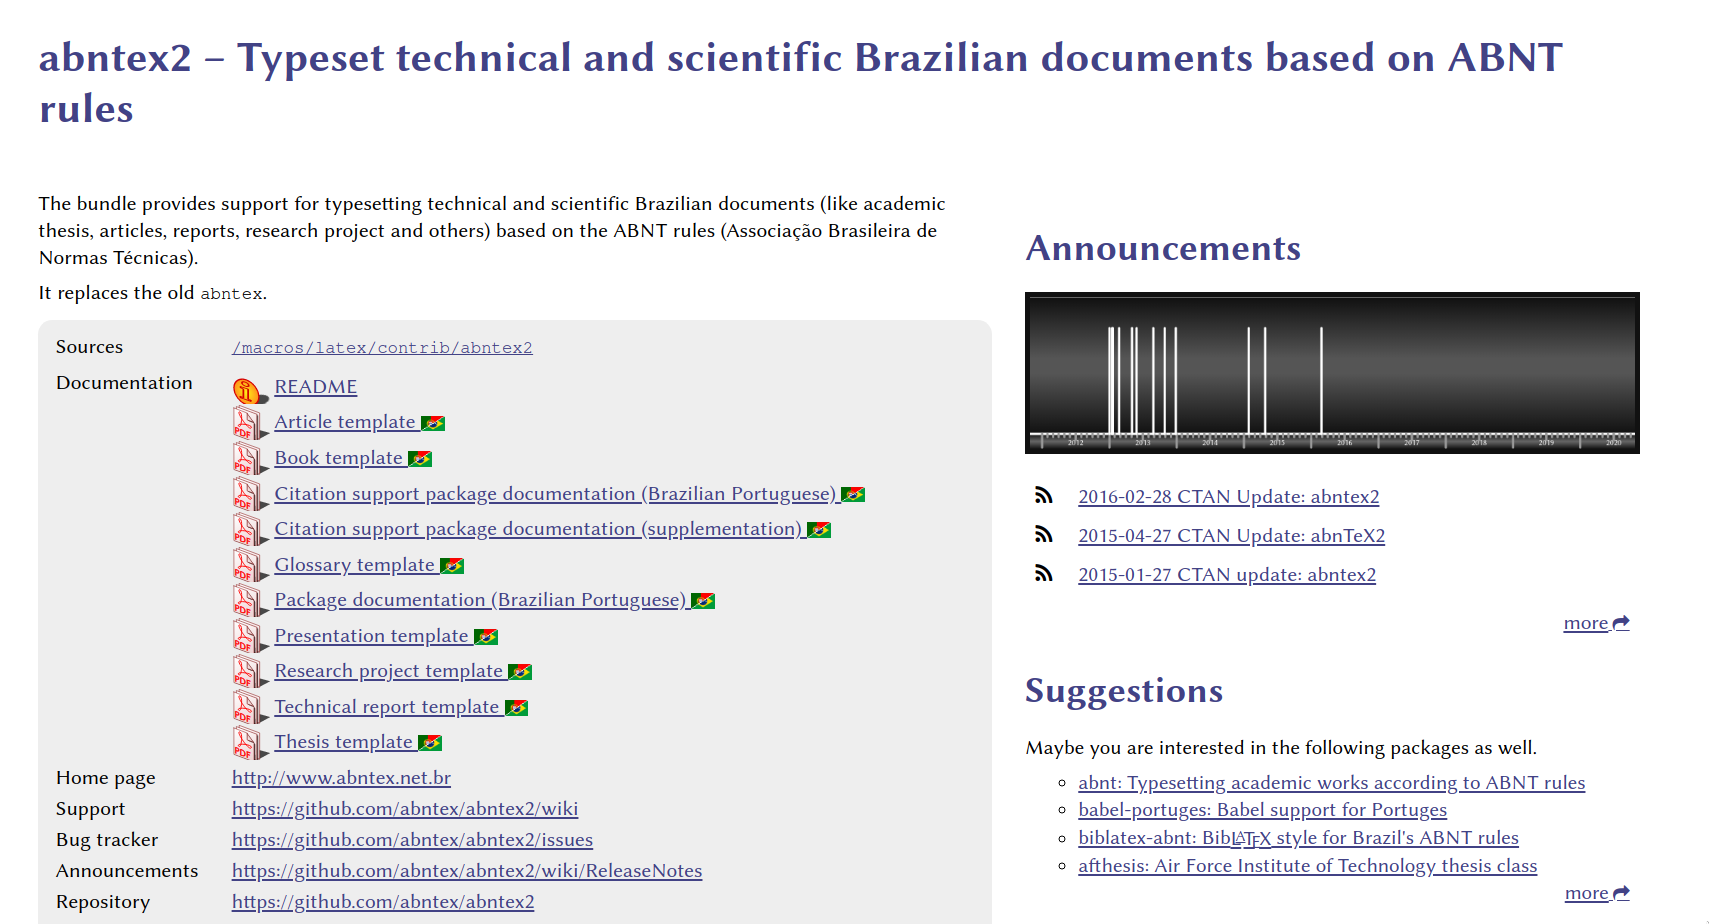
\includegraphics[scale=0.3]{Ilustracoes/1}
  \end{center}
  \legend{Fonte: os autores}
\end{figure}

Em geral, o CTAN é utilizado para se procurar a documentação de
pacotes. Muitas vezes, é mais interessante ler a documentação, para
entender um pacote, do que
procurar soluções prontas na internet. A longo prazo, é uma estratégia
melhor, para ter mais controle do seu documento.

\clearpage

\subsection{Overleaf}

Overleaf é uma plataforma, em que pode-se editar documentos em tempo
real e em grupo sem a necessidade de ter o \LaTeX instalado no
computador. Também, é possível acessar diversos templates, a partir do
site \footnote{https://www.overleaf.com/latex/templates}.

\begin{figure}[!htb]
  \caption{\label{site_overleaf} Site Overleaf, secção de templates}
  \begin{center}
    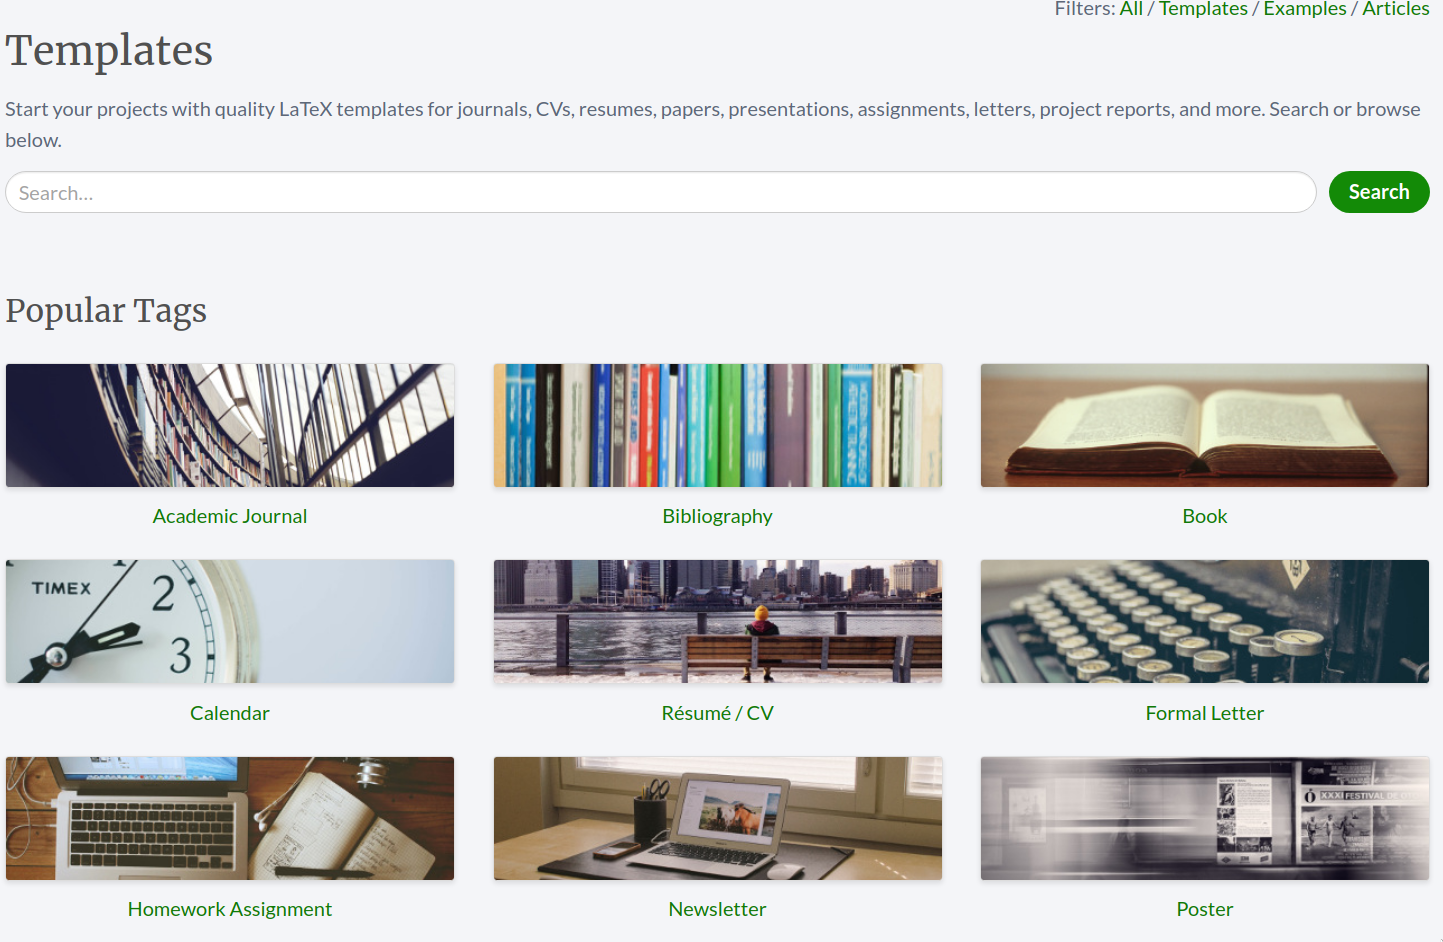
\includegraphics[scale=0.3]{Ilustracoes/2}
  \end{center}
  \legend{Fonte: os autores}
\end{figure}

O presente template do livro foi retirado do site Overleaf, bem como, estudado e
modificado pelo autor. Será explicado como fazer modificações e
personalizações mais a frente.

\subsection{Wikibook}

No site do wikibook há extensa documentação de comandos e exemplos de
como se utilizar o LaTeX
\footnote{https://en.wikibooks.org/wiki/LaTeX}.

\subsection{Projeto LaTeX}

O site do projeto LaTeX há documentação e publicações sobre os mais
recentes desenvolvimentos, e toda a cronologia do LaTeX
\footnote{https://www.latex-project.org/about/}. Assim, é uma fonte
bem avançada, e geralmente pouco utilizada pelos usuários; há mais
interesse para quem quer desenvolver pacotes etc.


\chapterimage{22.jpg} %33
\chapter{Comandos e Lógica Base do LaTeX}

\section{Variáveis Globais e Locais}

Ao escrever um documento, existem parâmetros que genéricos, e
universais. Por exemplo, o tamanho da fonte padrão, e os espaçamentos
entre linhas subsequêntes. A essas variáveis
dá-se o nome de \textbf{\scshape{Variáveis Globais}}.

Em contra-partida, há momentos do texto em que o comportamento global
é reescrito para uma formatação específica. Por exemplo, o tamanho da
letra do título de um capítulo, geralmente em negrito e com letras
aumentadas - quem sabe, até com outra fonte. A essas variáveis que
dependem do \textit{ambiente} em que está inserida, chama-as de
\textbf{\scshape{Variáveis Locais}}.

{\scshape{Na prática}}, não pensaremos na distinção das duas, quando estivermos
escrevendo um texto. Porém, conceitualmente é interessante entendermos
essa distinção, para que tenhamos uma melhor compreensão do mecanismo
do documento e pacotes.

Porém, imagine a situação que queiramos \textit{modular} o
comportamento de um pacote. Se observamos que o pacote possui
características locais, por exemplo, automaticamente, não
quebraremos nossa cabeça tentando alterar seu comportamento, com
variáveis globais. Pois, entenderíamos que seu comportamento tem de
ser alterado localmente. Por conseguinte, trabalharíamos dentro de seu
\emph{ambiente}. Vamos ver como isso se dá na prática!

\begin{center}
  \begin{forest}
    forked edges,
    for tree={draw,align=center,edge={-latex}}
    [Documento
    [Variáveis Globais
    [Fonte predominante]
    [Formato Seccionamento
    [Espaçamento entre \\ linhas e secções]
    ]]
    [Variáveis Locais
    [Ambientes
    [Imagens]
    [Tabelas]
    ]
    [Comandos
    [Negrito]
    [Itálico]
    [Fontes locais]
    ]]
    ]
  \end{forest}
\end{center}

\clearpage
\subsection{Ambientes e Comandos}

Todo comando possui duas formas, de um \textbf{ambiente} ou de um
\textbf{comando}. Aqui utilizamos a mesma palavra, comando, para duas
coisa distintas. Porém, ficará claro a distinção com um exemplo,

\subsubsection{Comando Ambiental}
\vspace{0.3cm}

\noindent Genericamente, se tem um \textbf{ambiente} da forma,

\begin{center}
\begin{verbatim}
\begin{comando}[opções]
  Texto, mais comandos.
\end{comando}
\end{verbatim}
\end{center}
\noident{Podemos \textbf{compor} de ambientes, os mais externos
  alterando os internos.}

\begin{center}
\begin{verbatim}
\begin{comando1}[opções]
  Texto da região afetada pelo comando 1, apenas.

  \begin{comando 2}[opções 2]
    Texto da região afetada pelos comandos 1 e 2.
       (...)
  \end{comando 2}

  Mais texto afetado pelo comando 1, apenas.
\end{comando1}
\end{verbatim}
\end{center}

\subsubsection{Ambiente de Imagens}
\vspace{.3cm}
\noident Observemos o caso das imagens, a grosso modo, usamos esse ambiente com
a seguinte estrutura,

\begin{center}
\begin{verbatim}
\begin{figure}[!htb]
  Site Overleaf, secção de templates
  \begin{center}
    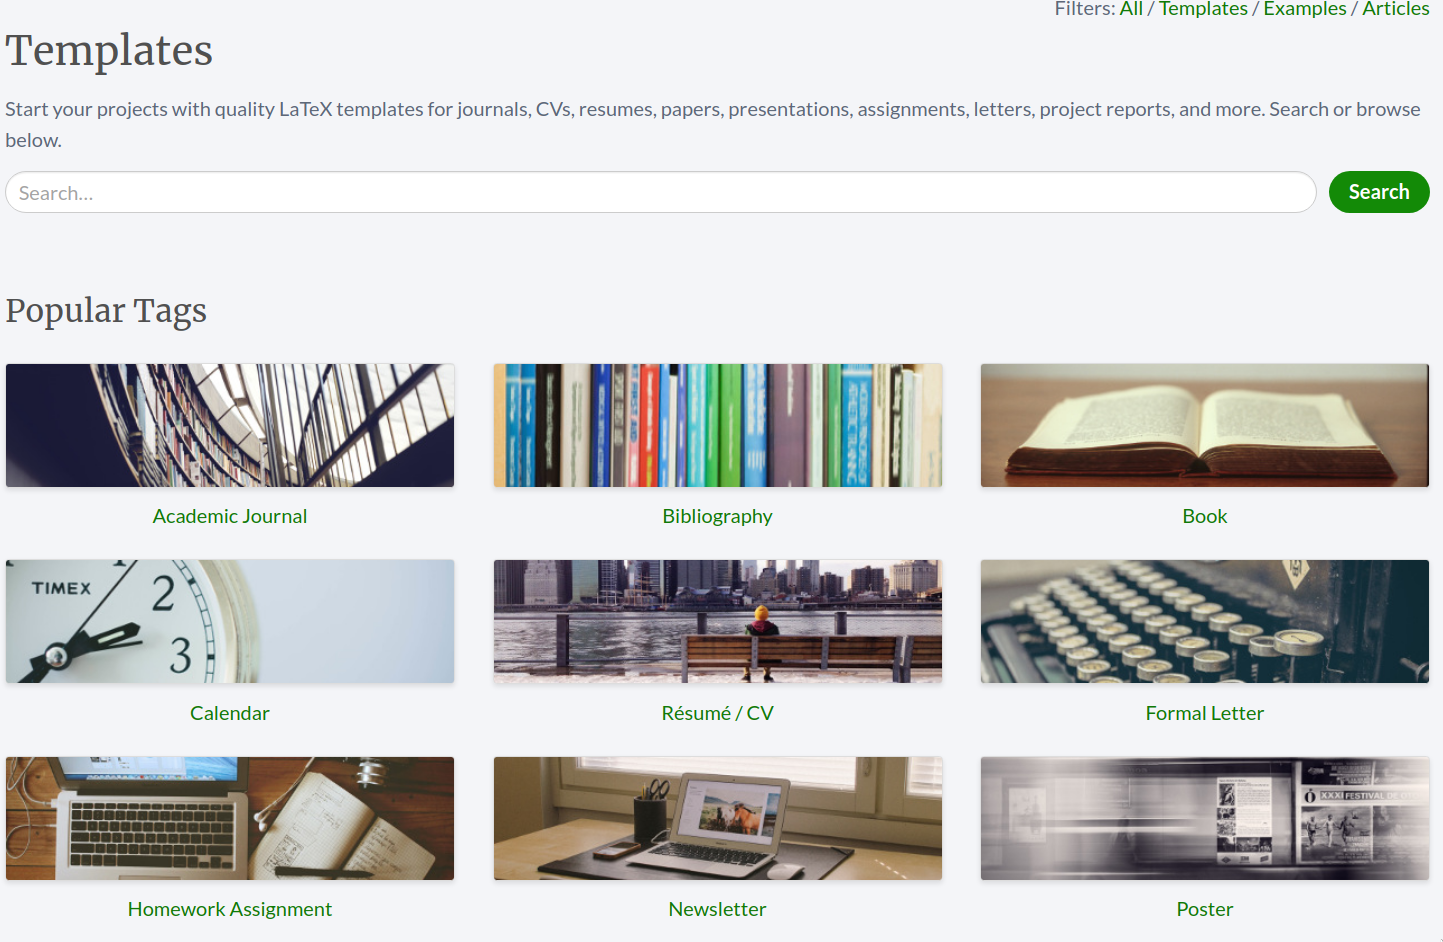
\includegraphics[scale=0.05]{Ilustracoes/2}
  \end{center}
  Fonte: os autores
\end{figure}
\end{verbatim}
\end{center}
\noident O resultado \footnote{Com uma pequena alteração, explicada a seguir},

\begin{figure}[!htb]
  \caption{\label{Exemplo1}\small{Site Overleaf, secção de templates}}

  \begin{center}
    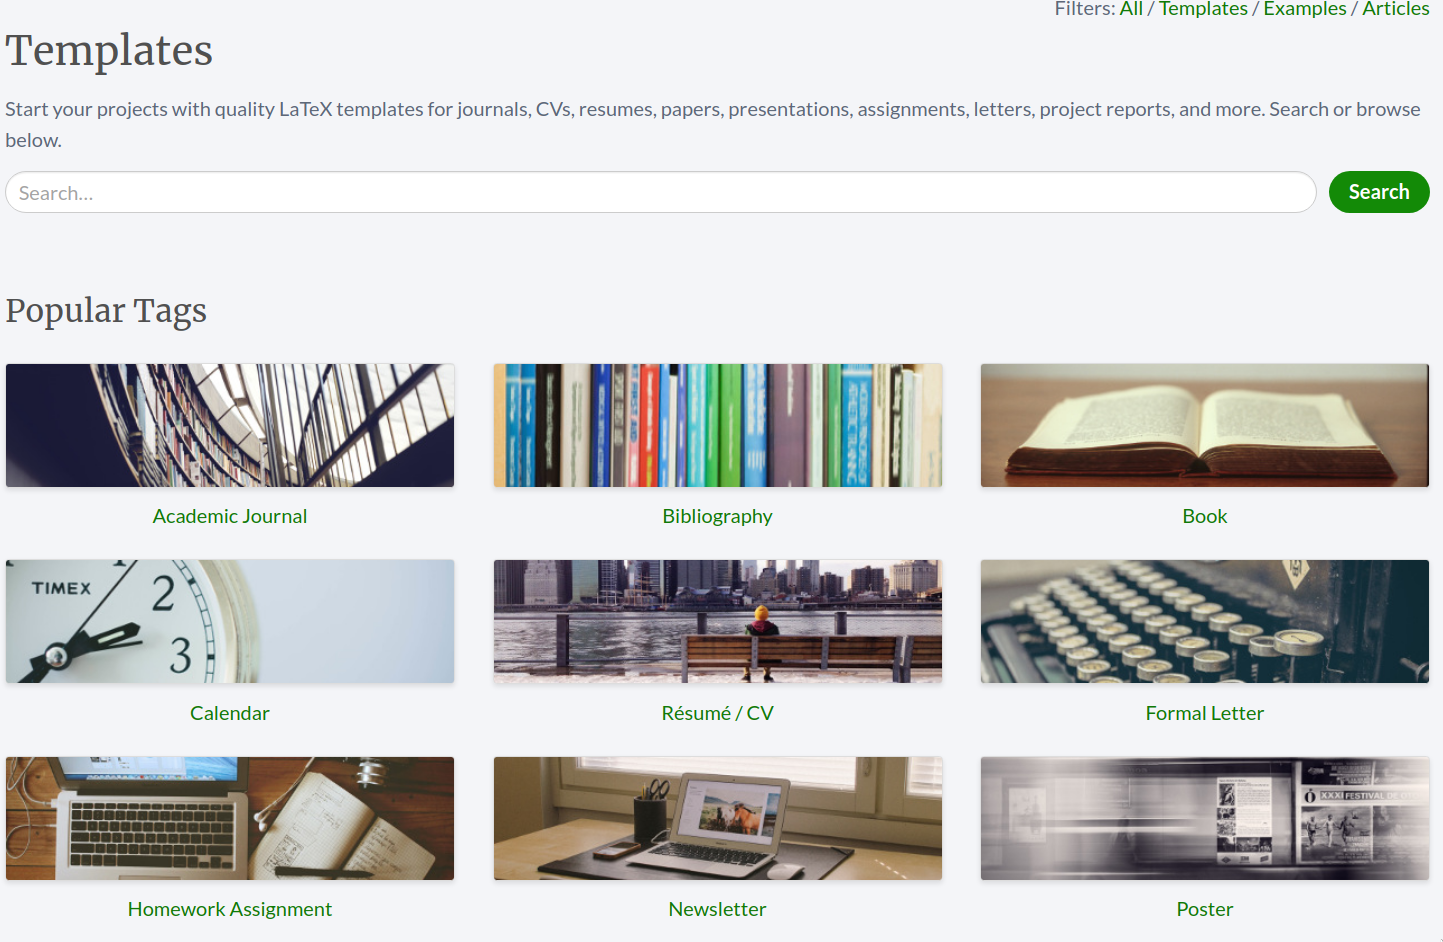
\includegraphics[scale=0.056]{Ilustracoes/2}
  \end{center}

  \legend{\small{Fonte: os autores}}
\end{figure}

\subsubsection{Comandos, em si}
\begin{myparindent}{0pt}
  \noindent Existe, porém, comandos que não dependem de um ambiente
  definidos por um começo e final. Eles possuem a simples forma,

  \begin{center}
\begin{verbatim}
\nome-do-comando[opções]{texto formatado pelo comando}
\end{verbatim}
  \end{center}
  \noident Assim é o caso do negrito, itálico, mudança de tamanho da
  fonte, inserções de imanges, entre outros. Estamos mudando, tanto nos comandos
  ambientais, quando nos comandos em si, o comportamento das variáveis
  globais.
  \vspace{0.4cm}

  \subsubsection{Composição de comandos}
  Os comandos podem ser \textbf{compostos} também. Isto é,
  \begin{center}
\begin{verbatim}
\comando1{texto-formato1 \comando2{texto-formato1e2} (...)}
\end{verbatim}
  \end{center}

  Digamos que queiramos que a fonte se torne do tipo smallcaps e em
  negrito,
\begin{verbatim}
\textbf{\scshape{Small Caps e Negrito}}
\end{verbatim}

  Teremos o resultado,

  \vspace{0.3cm}

  \textbf{\scshape{Small Caps e Negrito}}.

  \vspace{0.3cm}

  \subsubsection{Composição parcial}
  Note que poderíamos fazer as composições parcialmente, com a ordem da
  composição tendo importância,
\begin{verbatim}
\textbf{Um texto em negrito com eventual \scshape{Small Caps}}
{\scshape{Um texto em Small Caps com um eventual \textbf{Negrito}}}
\end{verbatim}

  Vejamos,

  \textbf{Um texto em negrito com eventual \scshape{Small Caps}}

  {\scshape{um texto em Small Caps com um eventual \textbf{Negrito}}}
\end{myparindent}
\clearpage
\subsection{Mistura de Comandos e Ambientes}
\begin{myparindent}{0pt}


  De fato, o que havíamos dado de comando para a \autoref{Exemplo1} da
  secção 2.1.1.2 Ambiente de Imagens, foi

\begin{verbatim}
\begin{figure}[!htb]
  \caption{\label{Exemplo1}\small{Site Overleaf, secção de templates}}

  \begin{center}
    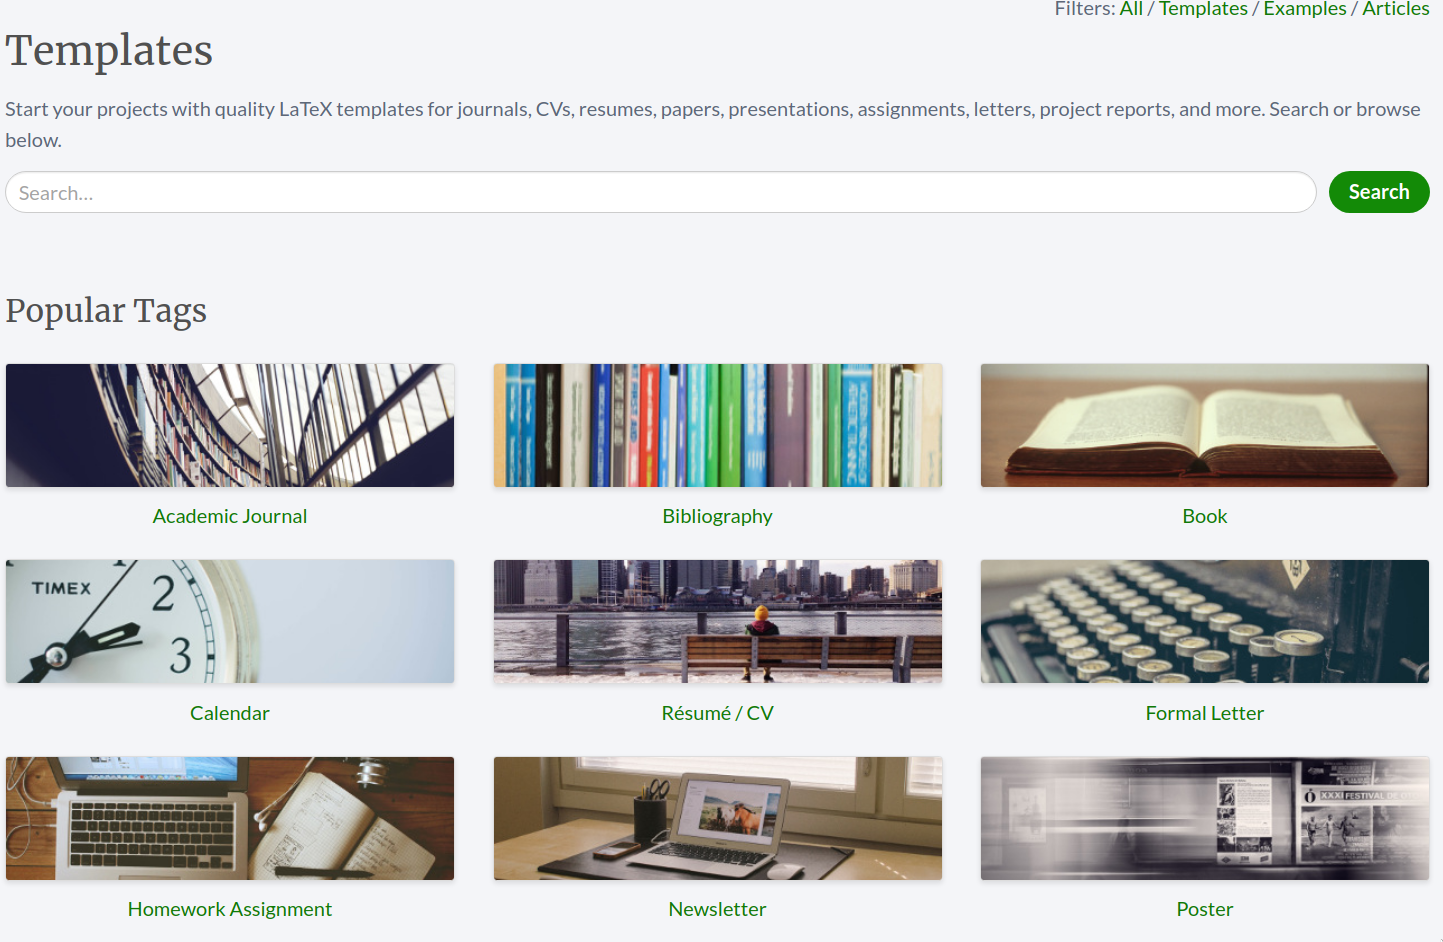
\includegraphics[scale=0.056]{Ilustracoes/2}
  \end{center}

  \legend{\small{Fonte: os autores}}
\end{figure}
\end{verbatim}

  Aqui temos um exemplo da composição entre comandos e comandos
  ambientais, pois dentro do ambiente \textbf{{\scshape{figure}}}, aparecem comandos
  como \small{\verb+\caption{\label{} texto-genêrico}+}. Também, vemos
  \small{\verb+\legend{\small{texto}}+}, e composições entre dois
  ambientes, como \textbf{{\scshape{figure}}} e
  \textbf{{\scshape{center}}}.

\end{myparindent}
\vspace{1cm}


Todas essas composições de \textit{funções} são comuns de
acontecer. E você, com um pouco de prática, as verá com a maior
naturalidade. Pois, o comportamento dessas composições é lógico e
unívoco. Não há como algo inesperado acontecer, incidentamente, sem
que um comando tenha sido escrito.

O intuito é que quem estiver usando \TeX{} foque menos na estrutura do
documento, e mais no seu conteúdo. Em geral, as variáveis globais já
terão definido a maior parte da estrutura do texto. E, essas são
customizáveis ao máximo, bem como, geralmente, já vem bem ajustadas em um template.

\vspace{1cm}
\section{\huge{Preâmbulo}}

No preâmbulo, localiza-se a customização das \textbf{variáveis
  globais}. Lá, é decidigo o tamanho da fonte global, seu estilo, os
espaçamentos entre linhas, entre secções, entre parágrafos, identações
etc. É muita informação pra se determinar, eu sei. Porém,
calma. Geralmente, não alteraremos grande parte das customizações em
um template ou em um pacote. Apenas temos a \textit{possibilidade}, se
quisermos.

O pacote ABNTeX2, por exemplo, é um dos pacotes que possui uma
identação própria; comandos típicos da ABNT, como um ambiente
\textbf{{\scshape{citacao}}} próprio para citações de mais de 3
linhas, o qual precisa ter uma formatação toda própria da ABNT. Coisa
que, nós, que utilizarmos o pacote, não precisaremos pensar
sobre. Apenas escreveremos, sem nos importar com a formatação resultante.

\begin{verbatim}
Assim já dizia o canto, de  St. Ambrose (340-397),

\begin{citacao}
  Surgamus ergo strenue!
  Gallus iacentes excitat,
  et somnolentos increpat,
  Gallus negantes arguit..
\end{citacao}

\end{verbatim}


\subsection{\Large{Exemplo de um preâmbulo}}

{\large{Essas informações inicial o documento .tex,}}
\begin{verbatim}

%%%% Declaração do estilo do documento, beamer (apresentações), articles
(artigos), book, letter etc. %%%%%

\documentclass[12pt, brazilian, twoside]{abntex2}

%%%%%%%%%% PREÂMBULO %%%%%%%%%%%%%%%%%%%

%%%%%%%%%%%%% Pacotes %%%%%%%%%
\usepackage{lipsum}             %%Pacore preenchedor de linguiça.
\usepackage{abntex2cite}        %%citação do tipo abnt
%\usepackage{asmath}            %%Pacote para formatação matemática
%\usepackage[portuguese]{babel} %%Pacote para português para
                                %%documentos que não são \documentclass{abntex2
%\usepackage[T1]{fontenc}       %%Reconhece acentos
\usepackage[utf8x]{inputenc}
\usepackage{lmodern}            %%Letras do tipo Latin Modern

%%%%%%%%%%% Formatação de espaçamento %%%%%%%

\setlength{\parindent}{4em}           %% Tamanho da identação
\setlength{\parskip}{1em}             %% Espaço entre parágrafos e texto
\renewcommand{\baselinestretch}{2.0}  %% Espaçamento entre linhas subsequêntes

%%%%%%%% Tudo que estiver depois do símbolo, %, é comentário - não é compilado.

\end{verbatim}

\subsubsection{\Large{Corpo do Documento}}
\vspace{0.3cm}
\begin{myparindent}{0pt}
{\large{Após o preâmbulo, todo o documento deve se encontrar dentro do
    ambiente \textbf{{\scshape{document}}}}}

\begin{verbatim}
\begin{document}

Corpo do documento

\end{document}
\end{verbatim}

\end{myparindent}
\clearpage

\subsubsection{\Large{Exemplo mais realista}}
\vspace{0.3cm}
\begin{myparindent}{0pt}
{\large{Um exemplo mais concreto da cara da estrutura de um texto,}}

\begin{verbatim}
\begin{document}
\chapter{Capítulo 1}

Texto

\section{Secção 1.1}

Texto

\subsecção{Subsecção 1.1.1}

Texto

\section{Secção 1.2}

Texto

\end{document}

\end{verbatim}

\end{myparindent}


{\large{Podemos utilizar o comando}} \verb+\lipsum[1] ; \lipsum[2-4]+
{\large{, et cetera, pra preencher o documento, dessa forma,}}

\begin{verbatim}

\begin{document}
\chapter{Capítulo 1}

\lipsum[1]

\section{Secção 1.1}

\lipsum[2-3]

\subsecção{Subsecção 1.1.1}

\lipsum[4]

\end{document}

\end{verbatim}

\clearpage

\section{Experimente}

Junte o preâmbulo dado como exemplo, e esse corpo do documento,
compile-os no texstudio, ou no Overleaf e veja o resultado. Você deve
ter algo do tipo,

\begin{figure}[!htb]
  \caption{\label{Documento} Compilando preâmbulo + corpo, com lipsum}
  \begin{center}
    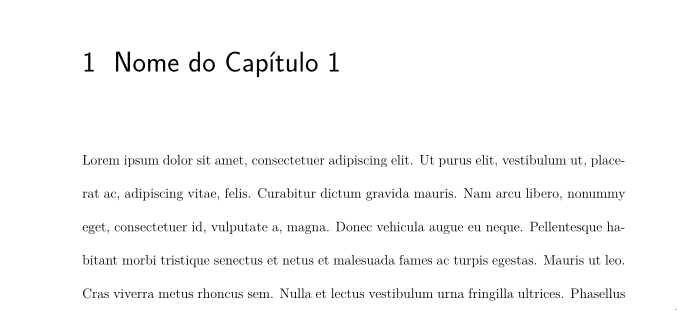
\includegraphics[scale=0.55]{Ilustracoes/3}
  \end{center}
  \legend{Fonte: os autores}
\end{figure}

Mude os parâmetros de espaçamento entre linhas, coloque uma imagem no
diretório do arquivo .tex, e utilize o modelo do livro para colocá-la
no documento.

Por fim, experimente! Agora, você já é capaz de entender a estrutura
geral de um template, de seus comandos, de modificar seus
parâmentros e aprender ativamente. Parabéns por chegar até
aqui. Desfrute de sua mais nova habilidade e conhecimentos!

{\scshape{Nos próximos capítulos}} nos aprofundaremos em comandos,
formatações de fórmulas matemáticas, o ambiente de tabelas, bem como,
como fazer uma apresentação, utilizando-se a classe de documentos Beamer!
%%%%%%%%%%%%%%%%%%%%%%%%%%%%%%%%%%%%%%



%%%%%%%%%% REFERÊNCIAS %%%%%%%%%%%%%%%%%%%
\chapterimage{5.jpg}
\bibliography{ref-bib}       %%puxa a bibliografia no diretório do
%% arquivo .tex, com nome 'ref-bib' (não
%% se põe se escreve a extensão .bib)



\end{document}

%%% Local Variables:
%%% mode: latex
%%% TeX-master: t
%%% End:
